\documentclass[tikz,border=2pt]{standalone}
\usepackage{amsmath}
\usepackage{tikz}
\usetikzlibrary{arrows.meta}

\begin{document}
% A bijection pairs every element of X with exactly one element of Y and vice versa, so reversing
% all arrows gives a function Y -> X: the inverse.
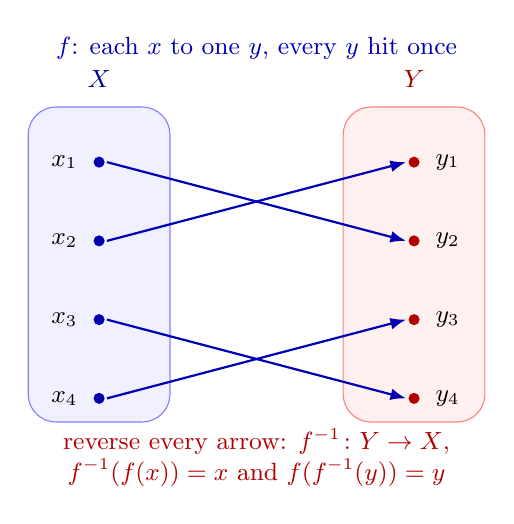
\begin{tikzpicture}[>={Latex[length=2mm]}, every node/.style={font=\small}]
	\draw[rounded corners=10pt, fill=blue!6, draw=blue!50] (-0.9,-2.1) rectangle (0.9,1.9);
	\draw[rounded corners=10pt, fill=red!6, draw=red!50] (3.1,-2.1) rectangle (4.9,1.9);
	\node[blue!60!black] at (0,2.25) {$X$};
	\node[red!60!black] at (4,2.25) {$Y$};
	\foreach \y/\l in {1.2/x_1, 0.2/x_2, -0.8/x_3, -1.8/x_4} {\fill[blue!70!black] (0,\y) circle (2pt); \node[left] at (-0.15,\y) {$\l$};}
	\foreach \y/\l in {1.2/y_1, 0.2/y_2, -0.8/y_3, -1.8/y_4} {\fill[red!70!black] (4,\y) circle (2pt); \node[right] at (4.15,\y) {$\l$};}
	\draw[->, blue!70!black, thick] (0.1,1.2) -- (3.9,0.2);
	\draw[->, blue!70!black, thick] (0.1,0.2) -- (3.9,1.2);
	\draw[->, blue!70!black, thick] (0.1,-0.8) -- (3.9,-1.8);
	\draw[->, blue!70!black, thick] (0.1,-1.8) -- (3.9,-0.8);
	\node[blue!70!black] at (2,2.65) {$f$: each $x$ to one $y$, every $y$ hit once};
	\node[red!70!black, align=center] at (2,-2.55) {reverse every arrow: $f^{-1}\colon Y\to X$,\\ $f^{-1}(f(x))=x$ and $f(f^{-1}(y))=y$};
\end{tikzpicture}
\end{document}
